\newpage
\section{line 类} %(fold)

变量 \tkzVar{line}{L} 保存一个用于存储直线对象的表。它是可选的，用户可自由选择自己的变量名（例如 \tkzname{Lines}）。
不过，为保持一致和便于阅读，推荐使用 \tkzVar{line}{L}。函数 \tkzFct{tkz-elements}{init\_elements()} 会自动重新初始化该表。


\subsection{创建直线}
\label{sub:creating_a_line}

要定义一条过两个已知点的直线，使用下面的构造函数：

\begin{mybox}
  \code{L.AB = line(z.A, z.B)} \hfill（简写，推荐）\\
  \code{L.AB = line:new(z.A, z.B)} \hfill（显式形式）
\end{mybox}

这会创建一个直线对象 \code{L.AB}，它表示：
\begin{itemize}
  \item 过点 \code{z.A} 和 \code{z.B} 的无限直线，以及
  \item 线段 $[AB]$，用于计算诸如中点或方向等属性。
\end{itemize}

\medskip

在内部，该对象存储这两个定义点，并从中推导出若干几何性质。

\subsection{直线的属性} %(fold)

考察 |L.AB = line(z.A, z.B)|

直线对象可访问以下属性：

\vspace{1em}
\bgroup
\catcode`_=12
\small
  \captionof{table}{直线的属性。}\label{line:attributes}
  \begin{tabular}{lll}
  \toprule
  \texttt{属性}   & \textbf{含义} & \texttt{参考}\\
  \midrule
  \tkzAttr{line}{type} & 始终为 \code{"line"}           &           \\
  \tkzAttr{line}{pa}   & 第一个点（例如 \code{z.A}）   &           \\
  \tkzAttr{line}{pb}   & 第二个点（例如 \code{z.B}）  &           \\
  \tkzAttr{line}{mid}  & 线段 $[AB]$ 的中点     &           \\
  \tkzAttr{line}{slope}& 相对于横轴的倾斜角 & [\ref{ssub:example_class_line}] \\
  \tkzAttr{line}{length} & 欧氏距离 $AB$ &  \ref{ssub:example_class_line}] \\
  \tkzAttr{line}{vec}   & 向量 $B - A$  &  [\ref{sec:class_vector}] \\
  \tkzAttr{line}{north\_pa}  & 位于 \code{pa} 北侧的辅助点 & [\ref{ssub:example_class_line}]  \\
    \tkzAttr{line}{north\_pb} & 位于 \code{pb} 北侧的辅助点 & -- \\
    \tkzAttr{line}{south\_pa} & 位于 \code{pa} 南侧的辅助点 & -- \\
    \tkzAttr{line}{south\_pb} & 位于 \code{pb} 南侧的辅助点 & -- \\
    \tkzAttr{line}{east}      & 位于线段东侧的辅助点 & -- \\
    \tkzAttr{line}{west}      & 位于线段西侧的辅助点 & -- \\
  \bottomrule
  \end{tabular}
\egroup


\subsubsection{示例：line 类的属性} %(fold)
\label{ssub:example_class_line}

\vspace{1em}
\begin{minipage}{.5\textwidth}
\directlua{
  init_elements()
  z.a = point(1, 1)
  z.b = point(5, 4)
  L.ab = line(z.a, z.b)
  z.m = L.ab.mid
  z.w = L.ab.west
  z.e = L.ab.east
  z.r = L.ab.north_pa
  z.s = L.ab.south_pb
  sl = L.ab.slope
  len = L.ab.length}
\begin{center}
\begin{tikzpicture}[scale = .5]
   \tkzGetNodes
   \tkzDrawPoints(a,b,m,e,r,s,w)
   \tkzLabelPoints(a,b)
   \tkzLabelPoint(r){north\_pa}
   \tkzLabelPoint(s){south\_pb}
   \tkzLabelPoint[below](m){mid}
   \tkzLabelPoint[right](w){west}
   \tkzLabelPoint[left](e){east}
   \tkzDrawLine(a,b)
   \tkzLabelSegment[above = 1em,sloped](a,b){ab = \pmpn{\tkzUseLua{len}}}
   \tkzLabelSegment[above=2em,sloped](a,b){(ab) 的斜率 =  \pmpn{\tkzUseLua{sl}}}
\end{tikzpicture}
\end{center}
\end{minipage}
\begin{minipage}{.5\textwidth}
\begin{tkzexample}[code only]
\directlua{
  init_elements()
  z.a = point(1, 1)
  z.b = point(5, 4)
  L.ab = line(z.a, z.b)
  z.m = L.ab.mid
  z.w = L.ab.west
  z.e = L.ab.east
  z.r = L.ab.north_pa
  z.s = L.ab.south_pb
  sl = L.ab.slope
  len = L.ab.length}
\end{tkzexample}
\end{minipage}

\subsubsection{关于直线对象属性的说明}

要取回直线对象 \tkzname{L.name} 的原始定义点，可使用以下任一方式：

\begin{itemize}
  \item 通过方法 \code{get(n)}，例如 \code{z.A, z.B = L.name:get()}，见 [\ref{ssub:method_line_get}]，
  \item 或直接通过其属性 \code{L.name.pa} 和 \code{L.name.pb}。
\end{itemize}
\newpage

\subsection{line 类的方法} %(fold)

下面是 \tkzNameObj{line} 对象的方法列表。返回结果可以是实数、点、直线、圆或三角形。所得三角形与下面定义的三角形类似。

\begin{minipage}{\textwidth}
\bgroup
\catcode`_=12
\small
\captionof{table}{line 类的方法。（第 1 部分）}\label{line:methods part 1}
\begin{tabular}{ll}
\toprule
\texttt{方法} & \texttt{参考}  \\
\midrule

\texttt{构造函数} & \\
\tkzMeth{line}{new(pt, pt)} &[\ref{sub:creating_a_line}; \ref{ssub:method_line_new_pt_pt}] \\

\midrule
\texttt{返回实数的方法} & \\
\midrule
\tkzMeth{line}{distance(pt)}  &  [\ref{ssub:method_line_distance}] \\
\midrule

\texttt{返回布尔值的方法} & \\

\tkzMeth{line}{on\_line(pt)}  & [\ref{ssub:method_on_line}] \\
\tkzMeth{line}{on\_segment(pt)} & [\ref{ssub:method_on_segment}] \\
\tkzMeth{line}{is\_parallel(L)}  & [\ref{ssub:method_line_is_parallel}]  \\
\tkzMeth{line}{is\_orthogonal(L)}  & [\ref{ssub:method_line_is_orthogonal}] \\
\tkzMeth{line}{is\_equidistant(pt)}  & [\ref{ssub:method_line_is_equidistant}]\\
\midrule

\texttt{返回字符串的方法} & \\
\midrule

\tkzMeth{line}{position(pt)}  & [\ref{ssub:method_line_position}] \\
\tkzMeth{line}{position\_segment(pt)} & [\ref{ssub:method_line_position_segment} \\
\tkzMeth{line}{where\_on\_line(pt)}  &  [\ref{ssub:method_line_where_on_line}] \\
\midrule

\texttt{返回点的方法} & \\
\midrule
\tkzMeth{line}{get(n)}       & [\ref{ssub:method_line_get}] \\
\tkzMeth{line}{random()}     & [\ref{ssub:method_line_random}] \\
\tkzMeth{line}{gold\_ratio()}&  [\ref{ssub:methode_imeth_line_gold__ratio}; \ref{sub:the_figure_pappus_circle}]  \\

\tkzMeth{line}{normalize()}        & [\ref{ssub:normalize}]\\
\tkzMeth{line}{normalize\_inv()}   & [\ref{ssub:normalize}]\\
\tkzMeth{line}{barycenter(r,r)}    & [\ref{ssub:barycenter_with_a_line}]\\
\tkzMeth{line}{point(r)}           & [\ref{ssub:method_point}]\\
\tkzMeth{line}{midpoint()}         & [\ref{ssub:method_line_midpoint}]\\
\tkzMeth{line}{harmonic\_int(pt)}  & [\ref{ssub:method_line_harmonic_int}]\\
\tkzMeth{line}{harmonic\_ext(pt)}  & [\ref{ssub:method_line_harmonic_ext}]\\
\tkzMeth{line}{harmonic\_both(r)}  & [\ref{ssub:harmonic_both}]\\
\tkzMeth{line}{harmonic(mode, pt)} & [\ref{ssub:harmonic}]\\
\tkzMeth{line}{report(d,pt)}       & [\ref{ssub:method_report}]\\
\tkzMeth{line}{collinear\_at(pt,k)}& [ex. \ref{ssub:method_line_collinear__at}]\\
\midrule

\texttt{返回直线的方法} & \\
\midrule
\tkzMeth{line}{ll\_from(pt)}    & [\ref{ssub_line_from_a_defined_line}] \\
\tkzMeth{line}{ortho\_from(pt)} & [\ref{ssubline_ortho_from}] \\
\tkzMeth{line}{mediator()}      &  [\ref{ssub:method_line_mediator}]\\
\tkzMeth{line}{equidistant\_with(L, <choice>)} & [\ref{ssub:method_line_equidistant_with}]\\
\tkzMeth{line}{swap\_line()}    & [\ref{ssub:method_line_swap__line} ; \ref{ssub:intersection_line_parabola_explained}] \\

\tkzMeth{line}{orthogonal\_at()} & \ref{ssub:method_line_orthogonal__at} \\
\bottomrule
\end{tabular}
\egroup
\end{minipage}

\begin{minipage}{\textwidth}
\bgroup
\catcode`_=12
\small
\captionof{table}{line 类的方法。（第 2 部分）}\label{line:methods part 2}
\begin{tabular}{lll}
\toprule
\texttt{方法} & \texttt{参考} & \\
\midrule
\texttt{返回三角形的方法} & \\
\midrule
\tkzMeth{line}{equilateral(<'swap'>)}    &  [\ref{ssub:method_line_equilateral};  \ref{ssub:object_rotation}]  \\

\tkzMeth{line}{isosceles(d,<'swap'>)}& [\ref{ssub:method_line_isosceles}]\\

\tkzMeth{line}{two\_angles(an,an)} & [\ref{ssub:triangle_with_two__angles}] \\
\tkzMeth{line}{school(<'swap'>)}     & [\ref{ssub:method_imeth_line_school_swap}] \\
\tkzMeth{line}{half(<'swap'>)}       & [\ref{ssub:method_imeth_line_half_swap}]\\
\tkzMeth{line}{s\_s(r,r<,'swap'>)}   & [\ref{ssub:triangle_with_three_given_sides}] \\
\tkzMeth{line}{sa\_(r,an<,'swap'>)}  & [\ref{ssub:_line_sas_d_an}]  \\
\tkzMeth{line}{\_as(r,an<,'swap'>)}  & [\ref{ssub:_line__as_d_an_swap}]  \\
\tkzMeth{line}{a\_s(r,an<,'swap'>)}  & [\ref{ssub:_line_a__s_d_an_swap}]\\
\tkzMeth{line}{s\_a(r,an<,'swap'>)}  & [\ref{ssub:_line_sa}]\\
\midrule
\texttt{返回神圣三角形的方法}&\\
\midrule
\tkzMeth{line}{gold(<'swap'>)}   &  [\ref{ssub:method_line_gold}] \\
\tkzMeth{line}{golden(<'swap'>)}  & （亦称 sublime）[\ref{ssub:method_line_golden}] \\
\tkzMeth{line}{golden\_gnomon(<'swap'>)} & [\ref{ssub:method_line_golden__gnomon}] \\
\tkzMeth{line}{pythagoras(<'swap'>)} & （亦称 egyptian）[\ref{ssub:_line_egyptian}] \\
\midrule
\texttt{返回圆的方法} &\\
\midrule
\tkzMeth{line}{circle()}  &  \\
\tkzMeth{line}{apollonius(r)}  &  [\ref{ssub:apollonius_circle_ma_mb_k}] \\
\tkzMeth{line}{LPP} & 即 c\_l\_pp(pt, pt) [\ref{ssub:c_l_pp}]  \\
\tkzMeth{line}{LLP} & 即 c\_ll\_p(L, pt) [\ref{ssub:method_c__ll__p}]  \\
\tkzMeth{line}{LLL(L, L)} & [\ref{ssub:method_LLL}]  \\
\midrule
\texttt{返回正方形的方法}&\\
\midrule
\tkzMeth{line}{square()}  &  [\ref{ssub:object_rotation}] \\
\midrule
\texttt{返回对象的方法} &\\
\midrule
\tkzMeth{line}{reflection(obj, ...)}  &  [\ref{ssub:reflection_of_object}] \\
\tkzMeth{line}{translation(obj, ...)} & [\ref{ssub:example_translation}] \\
\tkzMeth{line}{projection(obj)}  &  [\ref{ssub:example_projection_of_several_points}]\\
\tkzMeth{line}{projection\_ll(L, pts)}  & [\ref{ssub:method_line_projection__ll}] \\
\tkzMeth{line}{affinity(L, k, obj, ...)}  &  [\ref{ssub:method_line_affinity}] \\

\texttt{返回路径的方法} &\\
\midrule
\tkzMeth{line}{path(n)}  &  [\ref{ssub:line_path}] \\
\bottomrule
\end{tabular}
\egroup
\end{minipage}

\subsubsection{方法 \tkzMeth{line}{new(pt,pt)}} %(fold)
\label{ssub:method_line_new_pt_pt}

推荐使用诸如 \code{L.xx} 这样的写法，也推荐使用简写形式 \code{line(pt, pt)}。

\begin{tkzexample}[latex=.5\textwidth]
\directlua{
  init_elements()
  z.A = point(0, 0)
  z.B = point(4, 3)
  L.AB = line(z.A, z.B)}
\begin{center}
\begin{tikzpicture}
  \tkzGetNodes
  \tkzDrawLine(A,B)
  \tkzDrawPoints(A,B)
  \tkzLabelPoints(A,B)
\end{tikzpicture}
\end{center}
\end{tkzexample}

\subsection{返回实数}

本类只有一个方法


\subsubsection{方法 \tkzMeth{line}{distance(pt)}} %(fold)
\label{ssub:method_line_distance}

该方法给出一个点到一条直线的距离。

\vspace{1em}

\begin{tkzexample}[latex=.5\textwidth]
\directlua{
  init_elements()
  z.A = point(0, 0)
  z.B = point(4, 3)
  z.C = point(1, 5)
  L.AB = line(z.A, z.B)
  d = L.AB:distance(z.C)
  l = L.AB.length
  z.H = L.AB:projection(z.C)}
\begin{center}
\begin{tikzpicture}
\tkzGetNodes
\tkzDrawLines(A,B C,H)
\tkzDrawPoints(A,B,C,H)
\tkzLabelPoints(A,B,C,H)
\tkzLabelSegment[above right=2em,draw](C,H){%
  $CH = \tkzUseLua{d}$}
\tkzLabelSegment[below right=1em,draw](A,B){%
  $AB = \tkzUseLua{l}$}
\end{tikzpicture}
\end{center}
\end{tkzexample}

\subsection{返回布尔值}



 \subsubsection{方法 \tkzMeth{line}{on\_line(pt)}} %(fold)
\label{ssub:method_on_line}
%
该方法是 \tkzMeth{line}{position(pt)} 的布尔包装。

若点在直线上则返回 \code{true}，否则返回 \code{false}。

该方法也可用 \code{L:on\_line(pt)} 调用。

\texttt{注意： }
保留该方法是为了向后兼容。

\vspace{1em}

\begin{tkzexample}[latex=.5\textwidth]
\directlua{
  init_elements()
  local  function calc_distance(L, p)
    if L:on_line(p) then
      return point.abs(p - L.pa) / L.length
    else
      return 0
    end
  end
  z.A = point(0, 0)
  z.B = point(2, 4)
  z.X = point(3, 6)
  z.Y = point(2, 0)
  L.AB = line(z.A, z.B)
  dx = calc_distance(L.AB, z.X)
  dy = calc_distance(L.AB, z.Y)}
\begin{center}
  \begin{tikzpicture}
   \tkzGetNodes
   \tkzDrawLine(A,B)
   \tkzDrawPoints(A,B,X,Y)
   \tkzLabelPoints(A,B)
   \tkzLabelPoint(X){X: \tkzUseLua{dx}}
   \tkzLabelPoint(Y){Y: \tkzUseLua{dy}}
  \end{tikzpicture}
\end{center}
\end{tkzexample}



%
\subsubsection{方法 \tkzMeth{line}{on\_segment(pt)}} %(fold)
\label{ssub:method_on_segment}

上一个方法的变体；指示一个点是否位于线段上。


\tkzMeth{line}{position\_segment(pt)} 的布尔包装。

\texttt{返回： } 若 \tkzMeth{line}{position\_segment(pt)} 返回 \code{"ON"} 则为 \code{true}，
否则为 \code{false}。

\texttt{注意： } 保留以向后兼容。

\texttt{返回： }

\begin{itemize}
  \item 若点位于线段 $[pa,pb]$ 上则为 \code{true}，
  \item 否则为 \code{false}。
\end{itemize}

\vspace{1em}

\begin{tkzexample}[latex=.5\textwidth]
\directlua{
  init_elements()
  local  function inseg(L, p)
    if L:on_segment(p) then
      return "IN"
    else
      return "OUT"
    end
  end
  z.A = point(0, 0)
  z.B = point(2, 4)
  z.X = point(-1,-2)
  z.Y = point(1, 2)
  L.AB = line(z.A, z.B)
  dx = inseg(L.AB, z.X)
  dy = inseg(L.AB, z.Y)}
\begin{center}
  \begin{tikzpicture}
   \tkzGetNodes
   \tkzDrawLine(A,B)
   \tkzDrawPoints(A,B,X,Y)
   \tkzLabelPoints(A,B)
   \tkzLabelPoint(X){X: \tkzUseLua{dx}}
   \tkzLabelPoint(Y){Y: \tkzUseLua{dy}}
  \end{tikzpicture}
\end{center}
\end{tkzexample}

\subsubsection{方法 \tkzMeth{line}{is\_parallel(L)}} %(fold)
\label{ssub:method_line_is_parallel}

\vspace{1em}
\begin{tkzexample}[latex=.5\textwidth]
\directlua{
 init_elements()
 z.A = point(0, 0)
 z.B = point(4, 2)
 L.AB = line(z.A, z.B)
 z.C = point(1, 2)
 z.D = point(5, 4)
 L.CD = line(z.C, z.D)
 if L.AB:is_parallel(L.CD)
 then tkztxt = "parallel"
 else tkztxt = "no parallel"
 end}
\begin{center}
\begin{tikzpicture}
  \tkzGetNodes
  \tkzDrawLines(A,B C,D)
  \tkzDrawPoints(A,B,C,D)
  \tkzLabelPoints(A,B,C,D)
  \tkzLabelSegment[sloped,pos=.3](C,D){%
   $(CD)\ \tkzUseLua{tkztxt}\ (AB)$}
\end{tikzpicture}
\end{center}
\end{tkzexample}

\subsubsection{方法 \tkzMeth{line}{is\_orthogonal(L)}} %(fold)
\label{ssub:method_line_is_orthogonal}

\vspace{1em}

\begin{tkzexample}[latex=.5\textwidth]
\directlua{
 init_elements()
 z.A = point(0, 0)
 z.B = point(0, 4)
 L.AB = line(z.A, z.B)
 z.C = point(5, 4)
 L.BC = line(z.B, z.C)
 if L.AB:is_orthogonal(L.BC) then
   tkztxt = "orthogonal"
 else
   tkztxt = "no orthogonal"
 end}
\begin{center}
\begin{tikzpicture}
  \tkzGetNodes
  \tkzDrawLines(A,B B,C A,C)
  \tkzDrawPoints(A,B,C)
  \tkzLabelPoints(A,B,C)
  \tkzLabelSegment[sloped,pos=.3](B,C){%
    $(BC)\ \tkzUseLua{tkztxt}\ (AB)$}
\end{tikzpicture}
\end{center}
\end{tkzexample}

\subsubsection{方法 \tkzMeth{line}{is\_equidistant(pt)}} %(fold)
\label{ssub:method_line_is_equidistant}

一个点到定义该直线的两个点是否等距？

\begin{tkzexample}[latex=.5\textwidth]
\directlua{
  init_elements()
  z.A = point(0, 0)
  z.B = point(0, 4)
  z.C = point(4, 4)
  L.AC = line(z.A, z.C)
  if L.AC:is_equidistant(z.B) then
    tkztxt = "equidistant"
  else
    tkztxt = "no equidistant"
  end}
\begin{center}
    \begin{tikzpicture}
    \tkzGetNodes
    \tkzDrawLines(A,B B,C A,C)
    \tkzDrawPoints(A,B,C)
    \tkzLabelPoints(A,B,C)
    \tkzLabelSegment[sloped,pos=.3](A,C){%
      $B \ \tkzUseLua{tkztxt}\ of A\ and\ C$}
    \end{tikzpicture}
\end{center}
\end{tkzexample}

\subsection{返回字符串}

\subsubsection{方法 \tkzMeth{line}{position(obj[,EPS])}}
\label{ssub:method_line_position}

该方法对当前直线与另一对象之间的相对位置进行分类。
返回值是一个\emph{符号字符串}，其含义取决于 \code{obj} 的类型。
所有判断都在一个数值容差下进行。

\medskip
\textbf{参数：}
\begin{itemize}
  \item \code{obj}：一个 \tkzClass{point}、\tkzClass{line} 或 \tkzClass{circle}；
  \item \code{EPS}（可选）：数值容差。若省略，则使用 \code{tkz.epsilon}。
\end{itemize}

\medskip
\textbf{返回：}
\begin{itemize}
  \item 若 \code{obj} 是 \tkzClass{point}：若点在直线上（容差范围内）返回 \code{"ON"}，否则返回 \code{"OUT"}。
  \item 若 \code{obj} 是 \tkzClass{line}：返回 \code{line\_line\_position\_(self,obj,EPS)} 的结果。
  \item 若 \code{obj} 是 \tkzClass{circle}：返回 \code{line\_circle\_position\_(self,obj,EPS)} 的结果。
\end{itemize}

\medskip
\textbf{注意：}
该方法是一个基于 \code{getmetatable(obj)} 的分派器，默认使用 \code{tkz.epsilon}。


\subsubsection{方法 \tkzMeth{line}{position\_segment(pt)}}
\label{ssub:method_line_position_segment}

该方法确定一个点相对于直线对象所定义的线段
$[pa,pb]$ 的位置。

\texttt{参数： } \code{pt}：一个点。

\texttt{返回： }
\begin{itemize}
  \item 若点位于线段上（容差范围内）则为 \code{"ON"}，
  \item 否则为 \code{"OUT"}。
\end{itemize}

\texttt{注意： } 该方法使用数值容差 \code{tkz.epsilon}。


\subsubsection{方法 \tkzMeth{line}{where\_on\_line(pt)}}
\label{ssub:method_line_where_on_line}

该方法确定一个点 \code{pt} 沿一条直线的\emph{有向位置}，
该直线被视为从其第一个定义点 \code{pa} 指向第二个点
\code{pb}。

\medskip

该方法假定直线的方向为从 \code{pa} 到 \code{pb}。
它先检查该点是否在直线上（容差范围内）。
若不在，则该方法返回 \code{nil}。


\medskip

\paragraph{参数。}
\begin{itemize}
  \item \code{pt}：一个点。
\end{itemize}

\paragraph{返回。}
\begin{itemize}
  \item 若 \code{pt} 位于直线上、在 \code{pa} 的\emph{之前}，则为 \code{"BEFORE"}；
  \item 若 \code{pt} 位于线段 $[pa,pb]$ 上（即在 \code{pa} 与 \code{pb} 之间），则为 \code{"BETWEEN"}；
  \item 若 \code{pt} 位于直线上、在 \code{pb} 的\emph{之后}，则为 \code{"AFTER"}；
  \item 若 \code{pt} 不在直线上，则为 \code{nil}。
\end{itemize}

\paragraph{注意。}
\begin{itemize}
  \item 颠倒定义点 \code{pa} 与 \code{pb} 的顺序，会颠倒``BEFORE''与``AFTER''的含义。
  \item 该方法使用数值容差 \code{tkz.epsilon}。
\end{itemize}




\subsection{返回点}


\subsubsection{方法 \tkzMeth{line}{get()}}
\label{ssub:method_line_get}

该方法取回定义给定直线的两个点。例如在过某一特定点作另一直线的平行线时很有用：你需要两个点来确定方向。

\begin{itemize}
  \item \code{L.AB:get()} 返回两个点 \code{pa} 和 \code{pb}。
  \item \code{L.AB:get(1)} 返回第一个点 \code{pa}。
  \item \code{L.AB:get(2)} 返回第二个点 \code{pb}。
\end{itemize}

对于大多数由两个或更多点定义的几何对象（例如直线、三角形、圆），该方法都可用。它便于几何构造的复用与组合。


\begin{tkzexample}[latex=.35\textwidth]
  \directlua{
    init_elements()
    z.A = point(1, 1)
    z.B = point(2, 2)
    L.AB = line(z.A, z.B)
    z.C = L.AB.north_pa
    z.D = L.AB:ll_from(z.C):get(2)}

  \begin{tikzpicture}
    \tkzGetNodes
    \tkzDrawLines(A,B C,D)
    \tkzDrawPoints(A,B,C,D)
    \tkzLabelPoints(A,B,C,D)
  \end{tikzpicture}
\end{tkzexample}


\subsubsection{方法 \tkzMeth{line}{report(r,<pt>)}} %(fold)
\label{ssub:method_report}

\texttt{用途： } 该方法构造并返回一个 \tkzname{point}，它沿直线方向、与某个参考点相距给定距离 \( r \)。

\medskip

它推广了在线段上“量取一段长度”的概念。根据是否指定参考点，该方法要么从直线的第一个端点量起，要么从用户定义的起点量起。

\texttt{语法： }

\begin{center}
\begin{tabular}{lcl}
\code{L:report(r)} & $\rightarrow$ & 沿 \code{L.pb} 方向、距 \code{L.pa} 为 \( r \) 的点 \\
\code{L:report(r, pt)} & $\rightarrow$ & 平行于 \code{L}、距 \code{pt} 为 \( r \) 的点
\end{tabular}
\end{center}

\texttt{参数： }

\begin{description}
  \item[\code{r}]（数值）— 沿直线量取的有向距离。
  若 \(\,r>0\)，点位于从 \code{pa} 到 \code{pb} 的方向；
  若 \(\,r<0\)，则位于相反方向。
  \item[\code{pt}]（可选 \tkzname{point}）— 可选的参考点，从它开始量取距离。
\end{description}


\texttt{特殊情形： }

\begin{itemize}
  \item 若直线长度为零（即两个端点重合），则抛出错误。
  \item 负距离会在直线的反向延长线上产生点。
  \item 该方法对开放或有向直线（不仅是有限线段）都一致地适用。
\end{itemize}

\texttt{别名： } 为便于阅读，提供同义词 \code{point\_at\_distance}，尤其当几何意图是“沿某方向在给定距离处确定一个点”时。

\texttt{返回值： }
与所算出位置对应的新 \tkzname{point} 对象。


\vspace{1em}
\begin{tkzexample}[latex=.5\textwidth]
\directlua{
  init_elements()
  z.A = point(0, 0)
  z.B = point(4, 3)
  L.AB = line(z.A, z.B)
  z.M = point(0, 2)
  z.N = L.AB:report(2.5, z.M)
  z.O = L.AB:report(2.5)
  z.P = L.AB:report(-L.AB.length/3,z.M)}
\begin{center}
  \begin{tikzpicture}
  \tkzGetNodes
  \tkzDrawSegments(A,B P,N)
  \tkzDrawPoints(A,B,M,N,O,P)
  \tkzLabelPoints(A,B,M,N,O,P)
  \end{tikzpicture}
\end{center}
\end{tkzexample}

\subsubsection{方法 \tkzMeth{line}{barycenter(ka, kb)}} %(fold)
\label{ssub:barycenter_with_a_line}

该方法返回定义该直线的两个点的重心，权重为系数 \code{ka} 和 \code{kb}。

\medskip

在几何上，重心位于线段 $[AB]$（或其延长线）上，并根据系数的符号和比内分或外分该线段。


\begin{tkzexample}[latex=.5\textwidth]
\directlua{
 init_elements()
 z.A = point(0, -1)
 z.B = point(4, 2)
 L.AB = line(z.A, z.B)
 z.G = L.AB:barycenter(1, 2)}
\begin{center}
\begin{tikzpicture}
   \tkzGetNodes
   \tkzDrawLine(A,B)
   \tkzDrawPoints(A,B,G)
   \tkzLabelPoints(A,B,G)
\end{tikzpicture}
\end{center}
\end{tkzexample}

\subsubsection{方法 \tkzMeth{line}{point(r)} }%(fold)
\label{ssub:method_point}

该方法非常有用：它让你根据一个实参数 \code{r} 在直线上放置一个点。

\begin{itemize}
  \item 若 \code{r = 0}，结果为点 \code{pa}。
  \item 若 \code{r = 1}，结果为点 \code{pb}。
  \item 若 \code{r = 0.5}，结果为线段 $[AB]$ 的中点。
  \item \code{r} 可取任意值：负值把点放在 \code{pa} 之前，大于 1 的值把点放在 \code{pb} 之外。
\end{itemize}

对于所有由至少两个点定义的对象，都实现了该方法，四边形除外。


\begin{minipage}{.5\textwidth}
\directlua{
  init_elements()
  z.A = point(-1, -1)
  z.B = point(1, 1)
  L.AB = line(z.A, z.B)
  z.I = L.AB: point(0.75)
  z.J = L.AB: point(1.2)}
\begin{center}
  \begin{tikzpicture}[gridded]
  \tkzGetNodes
     \tkzDrawLine(A,J)
     \tkzDrawPoints(A,B,I,J)
     \tkzLabelPoints(A,B,I,J)
   \end{tikzpicture}
\end{center}
\end{minipage}
\begin{minipage}{.5\textwidth}
\begin{tkzexample}[code only]
\directlua{
  init_elements()
  z.A = point(-1, -1)
  z.B = point(1, 1)
  L.AB = line(z.A, z.B)
  z.I = L.AB: point(0.75)
  z.J = L.AB: point(1.2)}
\end{tkzexample}
\end{minipage}

\subsubsection{方法 \tkzMeth{line}{midpoint()}}
\label{ssub:method_line_midpoint}

该方法已由 \code{tkz.midpoint} 取代 [见 \ref{sub:midpoint_and_midpoints}]。

你可以用 \code{line} 对象的一个属性来获取线段的中点。

\begin{center}
  \code{z.M = L.AB.mid}
\end{center}

\medskip

不过，当直线对象尚未创建、且无需创建它时，独立函数 \code{tkz.midpoint(z.A, z.B)} 仍然方便高效。


\subsubsection{方法 \tkzMeth{line}{harmonic\_int(pt)}}
\label{ssub:method_line_harmonic_int}

给定直线上一个位于线段 $[AB]$ \emph{之外}的点，该方法返回线段上一个保持调和比的点。

\medskip

设 $AB$ 为一条直线，$D$ 为满足 $D \in (AB)$ 但 $D \not\in [AB]$ 的点。该方法返回一个点 $C \in [AB]$，使得：

\[
\frac{AC}{BC} = \frac{AD}{BD}
\]


这一构造在射影几何以及处理调和分割时特别有用。

\vspace{2em}
\begin{tkzexample}[vbox,overhang]
\directlua{
 init_elements()
 z.A = point(0, 0)
 z.B = point(6, 0)
 z.D = point(8, 0)
 L.AB = line(z.A, z.B)
 z.C = L.AB:harmonic_int(z.D)}
\begin{center}
  \begin{tikzpicture}
   \tkzGetNodes
   \tkzDrawLine(A,D)
   \tkzDrawPoints(A,B,C,D)
   \tkzLabelPoints(A,B,C,D)
  \end{tikzpicture}
\end{center}

\end{tkzexample}

\subsubsection{方法 \tkzMeth{line}{harmonic\_ext(pt)}}
\label{ssub:method_line_harmonic_ext}
该方法返回一个位于线段 $[AB]$ 之外的点，它与线段上一个给定点满足调和关系。

\medskip

设 $AB$ 为一条线段，$C$ 为 $[AB]$ 上一点（但不是中点）。该方法返回一个位于直线 $(AB)$ 上、但在线段 $[AB]$ \emph{之外}的点 $D$，使得：

\[
\frac{AC}{BC} = \frac{AD}{BD}
\]


这是方法 \tkzMeth{line}{harmonic\_int(pt)} 所执行操作的逆运算。

\subsubsection{方法 \tkzMeth{line}{harmonic\_both(k)}}
\label{ssub:harmonic_both}

该方法返回由 $AB$ 确定的直线上的两个点：

\begin{itemize}
  \item 一个点 $C$，位于线段 $[AB]$ \emph{内部}，
  \item 一个点 $D$，位于线段 $[AB]$ \emph{外部}，
\end{itemize}

  使得下面的调和比成立：

\[
\frac{AC}{BC} = \frac{AD}{BD} = k
\]


参数 \code{k} 表示所需的距离比。当你想同时构造给定线段的内调和共轭点和外调和共轭点时，该方法很有用。

\medskip

该方法按 \code{内部，外部} 的顺序返回这两个对应点。

\vspace{2em}
\begin{tkzexample}[vbox,overhang]
  \directlua{
   init_elements()
   z.A = point(0, 0)
   z.B = point(6, 0)
   L.AB = line(z.A, z.B)

   z.C, z.D = L.AB:harmonic_both(5)}
\begin{center}
  \begin{tikzpicture}
     \tkzGetNodes
     \tkzDrawLine(A,D)
     \tkzDrawPoints(A,B,C,D)
     \tkzLabelPoints(A,B,C,D)
  \end{tikzpicture}
\end{center}
\end{tkzexample}

\subsubsection{方法 \tkzMeth{line}{harmonic(mode, arg)}}
\label{ssub:harmonic}

该方法为调和分割提供统一接口。

\begin{itemize}
  \item \code{mode = "internal"} 返回内调和点。
  \item \code{mode = "external"} 返回外调和点。
  \item \code{mode = "both"} 返回两个调和点。
\end{itemize}

参数 \code{arg} 为：
\begin{itemize}
  \item 当 \code{mode} 为 \code{"internal"} 或 \code{"external"} 时是一个点，
  \item 当 \code{mode} 为 \code{"both"} 时是一个比。
\end{itemize}

\medskip
\noindent\textbf{示例}
\begin{verbatim}
H1      = L.AB:harmonic("internal",  z.P)
H2      = L.AB:harmonic("external",  z.P)
Hi, He  = L.AB:harmonic("both", 2)
\end{verbatim}




\subsubsection{方法 \tkzMeth{line}{gold\_ratio}}
\label{ssub:methode_imeth_line_gold__ratio}

该方法返回线段 $[AB]$ 上的一个点 $C$，它按\smallbf{黄金分割比}~$\varphi$ 分割该线段：

\[
\frac{AC}{CB} = \varphi = \frac{1 + \sqrt{5}}{2} \approx 1.618
\]


这一构造在需要和谐比例的设计、几何与美学中很有用。

\begin{tkzexample}[vbox]
\directlua{
   init_elements()
   z.A = point(0, 0)
   z.B = point(6, 0)
   L.AB = line(z.A, z.B)
   z.C = L.AB:gold_ratio()
   AC = tkz.length(z.A, z.C)
   BC = tkz.length(z.B, z.C)}

 AC/BC = \tkzUseLua{AC / BC}

 $\varphi = \tkzUseLua{(math.sqrt(5)+1)/2}$

\begin{center}
  \begin{tikzpicture}
     \tkzGetNodes
     \tkzDrawLine(A,B)
     \tkzDrawPoints(A,B,C)
     \tkzLabelPoints(A,B,C)
  \end{tikzpicture}
\end{center}

\end{tkzexample}

\subsubsection{方法 \tkzMeth{line}{normalize()} 与 \tkzMeth{line}{normalize\_inv()}} %(fold)
\label{ssub:normalize}

$ac = 1$ 且 $c\in [ab]$

$bd = 1$ 且 $d\in [ab]$

\vspace{1em}
\begin{tkzexample}[latex=.5\textwidth]
\directlua{
  init_elements()
  z.a = point(1, 1)
  z.b = point(5, 4)
  L.ab = line(z.a, z.b)
  z.c = L.ab:normalize()
  z.d = L.ab:normalize_inv()
}
\begin{center}
  \begin{tikzpicture}[gridded]
  \tkzGetNodes
  \tkzDrawSegments(a,b)
  \tkzDrawCircle(a,c)
  \tkzDrawPoints(a,b,c,d)
  \tkzLabelPoints(a,b,c,d)
  \end{tikzpicture}
\end{center}
\end{tkzexample}

\subsubsection{方法 \tkzMeth{line}{collinear\_at(pt,<r>)}} %(fold)
\label{ssub:method_line_collinear__at}

该方法返回一个点，它位于过给定点、平行于 $(AB)$ 的直线上。
所得点沿同一方向放置在与 $AB$ 长度成比例的距离处。

\medskip

若省略第二个参数 \meta{r}，默认为 $1$。
此时该方法产生一个与 $[AB]$ 长度和方向都相同的线段。

\medskip

除缩放因子形式外，该方法还接受一个选项表
\code{\{length =~$\ell$\}}，允许\emph{绝对地}指定距离 $CD$，
而与 $AB$ 无关。

\medskip

\textbf{示例解释：}
\begin{itemize}
  \item 若 \code{L.AB:collinear\_at(z.C)} 产生点 $E$，则 $CE = AB$ 且 $(AB) \parallel (CE)$。
  \item 若 \code{L.AB:collinear\_at(z.C, 0.5)} 产生点 $D$，则 $CD = 0.5 \cdot AB$ 且 $(AB) \parallel (CD)$。
  \item 若 \code{L.AB:collinear\_at(z.C, \{length = 2\})} 产生点 $F$，则 $CF = 2$（当前单位）且 $(AB) \parallel (CF)$。也可以使用负值。
\end{itemize}

这对于复制一个向量或把一个方向投影到平面中另一位置特别有用。

\vspace{1em}
\begin{tkzexample}[latex =.5\textwidth]
\directlua{
  init_elements()
  z.A = point(0, 0)
  z.B = point(4, 0)
  z.C = point(1, 3)
  L.AB = line(z.A, z.B)
  z.D = L.AB:collinear_at(z.C, .5)
  z.E = L.AB:collinear_at(z.C)
  z.F = L.AB:collinear_at(z.C, {length = -3})}
\begin{center}
\begin{tikzpicture}
 \tkzGetNodes
 \tkzDrawSegments(A,B C,E C,F)
 \tkzDrawPoints(A,B,C,D,E,F)
 \tkzLabelPoints(A,B,C,D,E,F)
\end{tikzpicture}
\end{center}
\end{tkzexample}


\subsubsection{方法 \tkzMeth{line}{orthogonal\_at(pt,<r>)}} %(fold)
\label{ssub:method_line_orthogonal__at}

该方法返回一个点，它位于过给定点、与直线 $(AB)$ \textbf{垂直}的直线上。

所得点沿与其正交的方向放置在与 $AB$ 长度成比例的距离处。
默认地，若省略第二个参数，因子为 $1$。

\medskip
除缩放因子形式外，该方法还接受一个选项表
\code{\{length =~$\ell$\}}，允许\emph{绝对地}指定距离 $CD$，
而与 $AB$ 无关。

\medskip

\texttt{示例解释：}
\begin{itemize}
  \item 若 \code{L.AB:orthogonal\_at(z.C)} 得到点 $E$，则 $CE = AB$ 且 $(AB) \perp (CE)$。
  \item 若 \code{L.AB:orthogonal\_at(z.C, 0.5)} 得到点 $D$，则 $CD = 0.5 \cdot AB$ 且 $(AB) \perp (CD)$。
  \item 若 \code{L.AB:orthogonal\_at(z.C, \{length = 2\})} 得到点 $F$，则 $CF = 2$（当前单位）且 $(AB) \perp (CF)$。也可以使用负值。
\end{itemize}

该方法有助于构造垂直向量，或构建诸如矩形、垂直平分线之类的几何图形。

\vspace{1em}
\begin{tkzexample}[latex =.5\textwidth]
\directlua{
  init_elements()
  z.A = point(0, 0)
  z.B = point(2, 0)
  z.C = point(1, 1)
  L.AB = line(z.A, z.B)
  z.D = L.AB:orthogonal_at(z.C, .5)
  z.E = L.AB:orthogonal_at(z.C)
  z.F = L.AB:orthogonal_at(z.C, {length = -3})}
\begin{center}
  \begin{tikzpicture}
    \tkzGetNodes
    \tkzDrawSegments(A,B C,E C,F)
    \tkzDrawPoints(A,B,C,D,E,F)
    \tkzLabelPoints(A,B,C,D,E,F)
  \end{tikzpicture}
\end{center}
\end{tkzexample}



\subsubsection{方法 \tkzMeth{line}{random()}}
\label{ssub:method_line_random}
该方法返回一个属于该线段的点。

\medskip
\texttt{语法： } \verb|z.M = L.AB:random()|


%%================================
\subsection{返回直线}
%%================================

\subsubsection{方法 \tkzMeth{line}{ll\_from(pt)}} %(fold)
\label{ssub_line_from_a_defined_line}

\medskip
\texttt{别名： } \code{parallel\_from}


\texttt{用途： } 该方法构造一个 \code{line} 类型的新对象，它平行于原直线且过给定点。

\medskip

与只返回一个沿同向平移的点的 \code{collinear\_at} 方法不同，\code{ll\_from} 返回一个完整的直线对象。这允许进行进一步运算，例如求交、投影，或沿该直线构造新点。

\medskip

\texttt{当你需要的是一个新的直线对象而非一个点时，使用本方法。}

 在 \code{ll\_from} 与 \code{collinear\_at} 之间如何选择，取决于具体语境，以及你是否需要把所得方向作为一个几何对象来处理。

\begin{minipage}{.5\textwidth}
\directlua{
  init_elements()
  z.A = point(1, 1)
  z.B = point(2, 2)
  L.AB = line(z.A, z.B)
  z.C = L.AB.north_pa
  z.D = L.AB.south_pa
  L.CD = line(z.C, z.D)
  _, z.E = L.CD:ll_from(z.B):get()}
\begin{center}
  \begin{tikzpicture}
  \tkzGetNodes
  \tkzDrawLines(A,B C,D B,E)
  \tkzDrawPoints(A,...,E)
  \tkzLabelPoints(A,...,E)
  \tkzMarkRightAngle(B,A,C)
  \tkzMarkSegments(A,C A,B A,D)
  \end{tikzpicture}
\end{center}
\end{minipage}
\begin{minipage}{.5\textwidth}
\begin{tkzexample}[code only]
\directlua{
  init_elements()
  z.A = point(1, 1)
  z.B = point(2, 2)
  L.AB = line(z.A, z.B)
  z.C = L.AB.north_pa
  z.D = L.AB.south_pa
  L.CD = line(z.C, z.D)
  _, z.E = L.CD:ll_from(z.B):get()}
\end{tkzexample}
\end{minipage}
%\begin{table}[h!]


\subsubsection{\texttt{collinear\_at} 与 \texttt{ll\_from} 方法的比较}

\bgroup
  \small
  \begin{tabular}{@{} l ll @{}}
  \toprule
  \smallbf{方面} & \code{collinear\_at(pt, r)} & \code{ll\_from(pt)} \\
  \midrule
  返回类型     & \code{point}                & \code{line} \\
  用途         & 平移得到的点            & 平行直线 \\
  输入           & 点、标量（可选）    & 点 \\
  默认标量  & \code{r = 1}                & 不适用 \\
  适用场景        & 向量位移         & 平行构造 \\
  \bottomrule
  \end{tabular}
\egroup


\subsubsection{方法 \tkzMeth{line}{ortho\_from(pt)}} %(fold)
\label{ssubline_ortho_from}

\texttt{别名： } \code{orthogonal\_from}


\texttt{用途： } 该方法构造一个 \code{line} 类型的新对象，它垂直于原直线且过给定点。

\medskip

与返回一个在垂直方向上相距给定距离的 \code{point} 的 \code{orthogonal\_at} 方法不同，\code{ortho\_from} 返回一个完整的 \code{line} 对象。这使它适合进一步的几何构造，例如求交、投影或作垂线。

\medskip

\texttt{当需要一条作为几何对象的垂线时，使用本方法。}

根据你需要的是一个点还是一条直线，在 \code{orthogonal\_at} 与 \code{ortho\_from} 之间选择。

\begin{minipage}{.5\textwidth}
  \directlua{
  init_elements()
  z.A = point(1, 1)
  z.B = point(3, 2)
  L.AB = line(z.A, z.B)
  z.C = point(1, 3)
  L.CD = L.AB:ortho_from(z.C)
  z.D = L.CD.pb}
  \begin{center}
  \begin{tikzpicture}
     \tkzGetNodes
     \tkzDrawLines(A,B C,D)
     \tkzDrawPoints(A,...,D)
     \tkzLabelPoints(A,...,D)
  \end{tikzpicture}
  \end{center}
\end{minipage}
\begin{minipage}{.5\textwidth}
\begin{tkzexample}[code only]
  \directlua{
  init_elements()
  z.A = point(1, 1)
  z.B = point(3, 2)
  L.AB = line(z.A, z.B)
  z.C = point(1, 3)
  L.CD = L.AB:ortho_from(z.C)
  z.D = L.CD.pb}
\end{tkzexample}
\end{minipage}

\subsubsection{\texttt{orthogonal\_at} 与 \texttt{ortho\_from} 的比较}


\begin{center}
  \bgroup
  \small
\begin{tabular}{@{} l ll @{}}
\toprule
\textbf{方面} & \texttt{orthogonal\_at(pt, r)} & \texttt{ortho\_from(pt)} \\
\midrule
返回类型     & \code{point}                   & \code{line} \\
用途         & 垂直位移     & 垂线 \\
输入           & 点、标量（可选）       & 点 \\
默认标量  & \code{r = 1}                   & 不适用 \\
适用场景        & 构造一个垂直点 & 构建一条垂线 \\
\bottomrule
\end{tabular}
\egroup
\end{center}

\subsubsection{方法 \tkzMeth{line}{mediator()}} %(fold)
\label{ssub:method_line_mediator}

在数学文献中（例如 \textit{MathWorld}），一条线段的\emph{mediator}——也称\emph{垂直平分线}——定义为过线段中点且垂直于该线段的直线。在三维几何中有时称为\emph{中垂面}。

\emph{mediator} 一词有历史渊源，尤其为 J. Neuberg 所使用（见 Altshiller-Court，1979，第 298 页）。在本宏包中，我选择采用法语词 \emph{médiatrice}，在此译作 \code{mediator}。

\medskip

该方法返回一个新的 \code{line} 对象，它垂直于原直线且过其中点。

\medskip

\texttt{别名： } 你也可以用别名 \code{perpendicular\_bisector()} 或 \code{bisector()} 调用本方法。

\vspace{1em}
\begin{tkzexample}[latex=.5\textwidth]
\directlua{
  init_elements()
  z.A = point(0,0)
  z.B = point(5,0)
  L.AB = line(z.A, z.B)
  L.med = L.AB:mediator()
  z.M = L.AB.mid
  z.x, z.y = L.med:get()}
\begin{center}
\begin{tikzpicture}
  \tkzGetNodes
  \tkzDrawLine(A,B)
  \tkzDrawSegments(x,y)
  \tkzDrawPoints(A,B,M)
  \tkzLabelPoints(A,B)
  \tkzLabelPoints[below left](x,y,M)
  \tkzMarkSegments(A,M M,B)
\end{tikzpicture}
\end{center}
\end{tkzexample}


\subsubsection{方法 \tkzMeth{line}{equidistant\_with(L, <choice>)}}
\label{ssub:method_line_equidistant_with}

该方法返回到本直线与到直线 \code{L} 等距的点的轨迹：
\begin{itemize}
  \item 若两直线平行，则为位于二者中间的平行线；
  \item 若它们相交，则为它们所成角的两条角平分线（过
        其交点）。
\end{itemize}
可选参数 \code{choice}（\code{1} 或 \code{2}）选择两条
角平分线中的一条。

\begin{tkzexample}[latex=.5\textwidth]
\directlua{
 init_elements()
 z.A = point(0, 0)
 z.B = point(4, 1)
 z.C = point(0, 3)
 z.D = point(4, 2)
 L.AB = line(z.A, z.B)
 L.CD = line(z.C, z.D)
 L.b1, L.b2 = L.AB:equidistant_with(L.CD)
 z.I = intersection(L.AB, L.CD)
 z.E = L.b1:report(3, z.I)
 z.F = L.b1:report(-3, z.I)
 z.G = L.b2:report(3, z.I)
 z.H = L.b2:report(-3, z.I)}
\begin{center}
\begin{tikzpicture}
 \tkzGetNodes
 \tkzDrawLines[add=.2 and 1.5](A,B C,D)
 \tkzDrawLines[red,add=0 and 0](E,F G,H)
 \tkzDrawPoints(A,B,C,D,I)
 \tkzLabelPoints(A,B,C,D,I)
\end{tikzpicture}
\end{center}
\end{tkzexample}

\subsubsection{方法 \tkzMeth{line}{collinear\_at\_distance(d)}}
\label{ssub:method_line_collinear_at_distance}

\texttt{描述： } 该方法创建一条平行于当前直线的新直线，相距一个有向距离 \texttt{d}。
\texttt{d} 的符号遵循通常约定：
\texttt{d > 0} 把直线移到有向线段 \(\overrightarrow{pa\,pb}\) 的\emph{左侧}，
\texttt{d < 0} 移到\emph{右侧}。

\medskip
\texttt{语法： } \verb|L' = L:collinear_at_distance(d)|

\medskip
\texttt{参数： } \texttt{d} — 有向偏移距离（实数，与坐标同单位）。

\medskip
\texttt{返回值： }

一个平行于 \texttt{L}、相距 \texttt{d} 的新 \tkzname{line} 对象。

\medskip
\texttt{用法示例： }

\begin{tkzexample}[latex=.4\textwidth]
\directlua{
  z.A = point(0, 0)
  z.B = point(5, 2)
  L.AB = line (z.A, z.B)
  L.n = L.AB:collinear_at_distance(-1)
  z.D, z.E = L.n:get()}
\begin{tikzpicture}[gridded,scale=.5]
\tkzGetNodes
\tkzDrawLines[blue](A,B)
\tkzDrawLines[red](D,E)
\tkzDrawPoints[red,size=4](A,B,D,E)
\tkzLabelPoints[red](A,B,D,E)
\end{tikzpicture}
\end{tkzexample}



\subsubsection{方法 \tkzMeth{line}{swap\_line}}
\label{ssub:method_line_swap__line}

\texttt{用途： }本方法并非供频繁使用，但在特定情形下可能有用。
创建一条直线时，它由两个点——\code{pa} 和 \code{pb}——定义，这两个点确定直线的方向。在某些几何构造中（尤其涉及圆锥曲线时），直线的方向会影响计算或方法的结果。

\medskip
\code{swap\_line()} 方法返回一个新的 \code{line} 对象，其定义点顺序颠倒，从而使直线方向反转。

\medskip

当涉及方向敏感的运算（例如投影、渐近线或有向相交判断）时，这一点尤其重要。

\vspace{1em}
\begin{tkzexample}[latex=7cm]
\directlua{
 init_elements()
 z.A = point(0, 0)
 z.B = point(2, -1)
 L.dir = line(z.A, z.B)
 L.dir = L.dir:swap_line()
 z.a = L.dir.pa
 z.b = L.dir.pb}
\begin{tikzpicture}
  \tkzGetNodes
  \tkzDrawSegments[cyan,thick,->](a,b)
  \tkzLabelPoints[below](A,B)
\end{tikzpicture}
\end{tkzexample}

\subsection{返回三角形}

\subsubsection{方法 \tkzMeth{line}{equilateral(<'swap'>)}}
\label{ssub:method_line_equilateral}

该方法以直线所定义的线段为底边构造一个等边三角形。

\medskip

该三角形三边相等，底边为从 \code{pa} 到 \code{pb} 的线段。构造遵循底边的方向。

\begin{itemize}
  \item 默认地，三角形按\emph{正向（逆时针）}构造：三角形顶点为 $A$、$B$、$C$，其中 $AB$ 为底边。
  \item 若给出可选参数 \code{"swap"}，则方向反转：三角形按反向（顺时针）顺序成为 $A$、$B$、$C$。
\end{itemize}

\medskip

该方法返回一个 \code{triangle} 对象。


\vspace{1em}
\begin{minipage}{.5\textwidth}
  \directlua{
   init_elements()
   z.A = point(0,0)
   z.B = point(4,0)
   L.AB = line(z.A, z.B)
   T.ABC = L.AB:equilateral()
   z.C = T.ABC.pc}
  \begin{center}
    \begin{tikzpicture}
    \tkzGetNodes
    \tkzDrawLine(A,B)
    \tkzDrawPolygon(A,B,C)
    \tkzMarkSegments(A,B B,C C,A)
    \tkzDrawPoints(A,B,C)
    \tkzMarkAngles(B,A,C C,B,A A,C,B)
    \tkzLabelPoints(A,B)
    \tkzLabelPoints[above](C)
    \end{tikzpicture}
  \end{center}
\end{minipage}
\begin{minipage}{.5\textwidth}
\begin{tkzexample}[code only]
\directlua{
 init_elements()
 z.A = point(0,0)
 z.B = point(4,0)
 L.AB = line(z.A, z.B)
 T.ABC = L.AB:equilateral()
 z.C = T.ABC.pc}
\end{tkzexample}
\end{minipage}

\subsubsection{方法 \tkzMeth{line}{isosceles(d, <'swap'>)}}
\label{ssub:method_line_isosceles}

该方法以直线所定义的线段为底边构造一个等腰三角形。

\medskip
参数 \code{d} 指定从底边每个端点延伸出的两条等边的长度。三角形按由 \code{pa} 到 \code{pb} 的方向所确定的默认方向构造。

\medskip

若给出可选参数 \meta{"swap"}，则三角形按相反方向构造（即顶点放在底边的另一侧）。

\medskip

该方法返回一个 \code{triangle} 对象。

\vspace{1em}
\begin{minipage}{.5\textwidth}
\directlua{
  init_elements()
  z.a = point(0, 0)
  z.b = point(3, 0)
  L.ab = line(z.a, z.b)
  T.abc = L.ab:isosceles(4)
  z.c = T.abc.pc}
\begin{center}
  \begin{tikzpicture}
  \tkzGetNodes
  \tkzDrawPolygons(a,b,c)
  \tkzDrawPoints(a,b,c)
  \tkzLabelPoints[above](c)
  \tkzLabelPoints(a, b)
  \tkzLabelSegment[right](b,c){$4$}
   \tkzLabelSegment[left](a,c){$4$}
  \end{tikzpicture}
\end{center}
\end{minipage}
\begin{minipage}{.5\textwidth}
\begin{tkzexample}[code only]
\directlua{
  init_elements()
  z.a = point(1, 2)
  z.b = point(3, 1)
  L.ab = line(z.a, z.b)
  T.abc = L.ab:isosceles(4)
  z.c = T.abc.pc}
\end{tkzexample}
\end{minipage}

\subsubsection{方法 \tkzMeth{line}{school(<'swap'>)}}
\label{ssub:method_imeth_line_school_swap}
\code{school} 三角形是一个直角三角形，三个角分别为 $30^\circ$、$60^\circ$、$90^\circ$——在初等几何构造中常用。

\medskip

默认地，$30^\circ$ 角位于直线的第一个点（\code{pa}），$60^\circ$ 角位于第二个点（\code{pb}）。使用可选参数 \meta{"swap"} 会颠倒这种放置，交换两个底角。

\medskip


要反转三角形的方向（即按反向构造），只需颠倒定义直线的点的顺序，例如：
\code{L.AB = line(z.B, z.A)}。

\vspace{1em}
\begin{minipage}{.5\textwidth}
\directlua{
  init_elements()
  z.A = point(0, 0)
  z.B = point(4, 0)
  L.AB = line(z.A, z.B)
  T.ABC = L.AB:school()
  z.C = T.ABC.pc}
\begin{center}
\begin{tikzpicture}
  \tkzGetNodes
  \tkzDrawPolygons(A,B,C)
  \tkzDrawPoints(A,B,C)
  \tkzLabelPoints(A,B)
  \tkzLabelPoints[above](C)
  \tkzMarkAngle[red](C,B,A)
  \tkzMarkAngle[red](B,A,C)
  \tkzMarkAngle[red](A,C,B)
  \tkzLabelAngle[red,
   pos=.5](A,C,B){$\scriptstyle\pi/2$}
  \tkzLabelAngle[red,
    pos=.7](B,A,C){$\scriptstyle\pi/6$}
  \tkzLabelAngle[red,
     pos=.5](C,B,A){$\scriptstyle\pi/3$}
\end{tikzpicture}
\end{center}

\end{minipage}
\begin{minipage}{.5\textwidth}
\begin{tkzexample}[code only]
\directlua{
  init_elements()
  z.A = point(0, 0)
  z.B = point(4, 0)
  L.AB = line(z.A, z.B)
  T.ABC = L.AB:school()
  z.C = T.ABC.pc}
\end{tkzexample}
\end{minipage}

\subsubsection{方法 \tkzMeth{line}{half(<'swap'>)}}
\label{ssub:method_imeth_line_half_swap}

该方法构造一个直角三角形，其两条直角边之比为 $1:2$。

\medskip

默认地，直角位于直线的第一个点（\code{pa}）。若给出可选参数 \meta{"swap"}，则直角放在第二个点（\code{pb}）。

\medskip

这类三角形有助于构造简单几何构型或说明特殊三角形情形。

\vspace{1em}
\begin{minipage}{.5\textwidth}
\directlua{
  init_elements()
  z.A = point(0, 0)
  z.B = point(4, 0)
  L.AB = line(z.A, z.B)
  T.ABC = L.AB:half('swap')
  z.C = T.ABC.pc}
\begin{center}
\begin{tikzpicture}
  \tkzGetNodes
  \tkzDrawPolygons(A,B,C)
  \tkzDrawPoints(A,B,C)
  \tkzLabelPoints(A,B)
  \tkzLabelPoints[above](C)
  \tkzLabelAngle[red,
   pos=.5](B,A,C){$\scriptstyle\pi/2$}
   \tkzLabelSegment(A,B){$AB =  2 AC$}
\end{tikzpicture}
\end{center}

\end{minipage}
\begin{minipage}{.5\textwidth}
\begin{tkzexample}[code only]
\directlua{
  init_elements()
  z.A = point(0, 0)
  z.B = point(4, 0)
  L.AB = line(z.A, z.B)
  T.ABC = L.AB:half('swap')
  z.C = T.ABC.pc}
\end{tkzexample}
\end{minipage}

\subsubsection{方法 \tkzMeth{line}{two\_angles(an, an)}}
\label{ssub:triangle_with_two__angles}

该方法通过在给定线段每个端点处指定两个角来构造三角形。它通过确定第三个顶点使内角和为 $180^\circ$，从而补全三角形。

\medskip

所给两个角分别施加在直线的端点 \code{pa} 和 \code{pb} 处。所得三角形通过把这些角的边延长至相交来确定。

\medskip

该方法对应经典的 ASA 构造（\textit{角–边–角}），也可用别名 \code{asa} 或 \code{a\_a} 调用。

\vspace{1em}

\begin{minipage}{.35\textwidth}
\directlua{
  init_elements()
  z.A = point(0, 0)
  z.B = point(4, 0)
  L.AB = line(z.A, z.B)
  T.ABC = L.AB:two_angles(math.pi / 6,2 *  math.pi / 5)
  z.C = T.ABC.pc}
\begin{center}
  \begin{tikzpicture}
     \tkzGetNodes
     \tkzDrawPolygons(A,B,C)
     \tkzDrawPoints(A,B,C)
     \tkzLabelPoints(A,B)
     \tkzLabelPoints[above](C)
     \tkzMarkAngle[red](C,B,A)
     \tkzMarkAngle[red](B,A,C)
     \tkzLabelAngle[red,
      pos=1.3](C,B,A){$\scriptstyle2\pi/5$}
     \tkzLabelAngle[red,
      pos=1.3](B,A,C){$\scriptstyle\pi/6$}
  \end{tikzpicture}
\end{center}
\end{minipage}
\begin{minipage}{.65\textwidth}
\begin{tkzexample}[code only]
\directlua{
 init_elements()
 z.A = point(0, 0)
 z.B = point(4, 0)
 L.AB = line(z.A, z.B)
 T.ABC = L.AB:two_angles(math.pi / 6,2 *  math.pi / 5)
 z.C = T.ABC.pc}
\end{tkzexample}
\end{minipage}

\subsubsection{方法 \tkzMeth{line}{s\_s(d, d)}}
\label{ssub:triangle_with_three_given_sides}

该方法给定三角形三边长度（底边及与之相邻的两边）来构造三角形。

\medskip

三角形的底边由直线对象（例如 \code{L.AB}）定义，它确定 \code{pa} 与 \code{pb} 之间的线段。两个参数 \code{d} 表示其余两边的长度。

\medskip

这一构造对应经典的 \code{SSS} 情形（\textit{边–边–边}），该方法也可用别名 \code{s\_s} 或 \code{sss} 调用。

\vspace{1em}

\begin{minipage}{.5\textwidth}
\directlua{
  init_elements()
  z.A = point(0, 0)
  z.B = point(5, 0)
  L.AB = line(z.A, z.B)
  T.ABC = L.AB:s_s(3, 4)
  z.C = T.ABC.pc}
  \begin{center}
    \begin{tikzpicture}[gridded]
      \tkzGetNodes
      \tkzDrawPolygons(A,B,C)
      \tkzDrawPoints(A,B,C)
      \tkzLabelPoints(A,B)
      \tkzLabelPoints[above](C)
    \end{tikzpicture}
  \end{center}
\end{minipage}
\begin{minipage}{.5\textwidth}
\begin{tkzexample}[code only]
\directlua{
  init_elements()
  z.A = point(0, 0)
  z.B = point(5, 0)
  L.AB = line(z.A, z.B)
  T.ABC = L.AB:s_s(3, 4)
  z.C = T.ABC.pc}
\end{tkzexample}
\end{minipage}

\subsubsection{方法 \tkzMeth{line}{sa\_(d, an, <'swap'>)}}
\label{ssub:_line_sas_d_an}

该方法由给定底边（直线）、一条边长以及该边与底边之间的角来构造三角形。

\medskip

它对应经典的 \code{SAS} 情形（\textit{边–角–边}）。长度为 \code{d} 的边放在底边的第一个点 \code{pa} 处，角 \code{an}（度）在该边与底边之间形成。

\medskip

若给出可选参数 \meta{"swap"}，则该边和角改为从第二个点 \code{pb} 施加，相当于把三角形沿底边镜像。

\vspace{1em}
\directlua{
  init_elements()
  z.A = point(0, 0)
  z.B = point(5, 0)
  L.AB = line(z.A, z.B)
  T.ABD = L.AB:sa_(3, tkz.tau / 5)
  z.D = T.ABD.pc}
  \begin{center}
    \begin{tikzpicture}[gridded]
      \tkzGetNodes
      \tkzDrawPolygons(A,B,D)
      \tkzDrawPoints(A,B,D)
      \tkzLabelPoints(A,B)
      \tkzLabelPoints[above](D)
    \end{tikzpicture}
  \end{center}

\subsubsection{方法 \tkzMeth{line}{\_as(d, an,<'swap'>)}}
\label{ssub:_line__as_d_an_swap}

该方法与 \code{sa\_} 相对应。它用给定底边（直线）、一条长度为 \code{d} 的边以及与该边相邻的角 \code{an} 来构造三角形，但这次从底边的第二个点 \code{pb} 量起。

\medskip

这一构造仍对应经典的 \code{SAS} 情形（\textit{边–角–边}），但从底边端点反向施加。

\medskip

若给出可选参数 \meta{"swap"}，则三角形按反向（顺时针）构造，这在构造镜像构型时可能有用。


\subsubsection{方法 \tkzMeth{line}{s\_a(d, an, <'swap'>)}}
\label{ssub:_line_sa}

该方法由给定底边（直线）、一条长度为 \code{d} 的边以及该边所对的角 \code{an} 来构造三角形。

\medskip

这一构造对应经典的 \code{SSA} 情形（\emph{边–边–角}），它是歧义的：根据边和角的取值，结果可能为：

\begin{itemize}
  \item 没有三角形（无效构型），
  \item 恰有一个三角形，
  \item 或可能有两个三角形。
\end{itemize}

\medskip

当可能有两个三角形时，该方法默认返回在底边处角较大的那个。若给出可选参数 \meta{"swap"}，则返回第二个解。

\vspace{1em}

\directlua{
  init_elements()
  z.A = point(0, 0)
  z.B = point(5, 0)
  L.AB = line(z.A, z.B)
  T.ABE = L.AB:s_a(4, math.pi / 5)
  z.E = T.ABE.pc
  T.ABD = L.AB:s_a(4, math.pi / 5,'swap')
  z.D = T.ABD.pc
  }
\begin{center}
\begin{tikzpicture}[gridded]
 \tkzGetNodes
 \tkzDrawPolygons(A,B,E A,B,D)
 \tkzDrawPoints(A,B,E,D)
 \tkzLabelPoints(A,B)
 \tkzLabelPoints[above](E,D)
\end{tikzpicture}
\end{center}

\subsubsection{方法 \tkzMeth{line}{a\_s(d,an,<'swap'>)}}
\label{ssub:_line_a__s_d_an_swap}

\subsubsection{由直线构造三角形的方法小结}

\begin{center}
  \bgroup
  \small
\begin{tabular}{@{} llll @{}}
\toprule
\smallbf{方法} & \smallbf{类型} & \smallbf{参数} & \smallbf{角的构型} \\
\midrule
\code{equilateral()}   & 等边 & 无               & $60^\circ$ – $60^\circ$ – $60^\circ$ \\
\code{isosceles(d)}    & 等腰   & 一条边           & 两个相等的角 \\
\code{school()}        & 直角       & 无               & $30^\circ$ – $60^\circ$ – $90^\circ$ \\
\code{half()}          & 直角       & 无               & 一个角满足 $\tan\theta = 1/2$ \\
\code{two\_angles(a,b)}& ASA         & 两个角         & 端点处两个角 \\
\code{s\_s(d,d)}       & SSS         & 两条边          & 已知三边 \\
\code{sa\_(d,an)}      & SAS         & 边 + 在 \code{pa} 处的角 & 第一点处的夹角 \\
\code{\_as(d,an)}      & SAS         & 边 + 在 \code{pb} 处的角 & 第二点处的夹角 \\
\code{s\_a(d,an)}      & SSA         & 边 + 对角 & 可能歧义 \\
\bottomrule
\end{tabular}
\egroup
\end{center}

\subsection{返回神圣三角形}

赋予这些三角形的名称是传统或象征性的，可能与标准数学文献中的用法不同。

\vspace{1em}
\begin{tabular}{@{}ll@{}}
\toprule
\smallbf{名称（方法）} & \smallbf{定义 / 性质} \\
\midrule
\tkzMeth{line}{gold()} &
直角三角形，$c/b = \sqrt{\varphi}$；黄金矩形的一半 \\
\addlinespace
\tkzMeth{line}{golden()} &
等腰三角形，$b/c = \varphi$，角 $\alpha = \beta = \dfrac{2\pi}{5}$；\\
& 亦称：sublime 三角形、欧几里得三角形 \\
\addlinespace
\tkzMeth{line}{golden\_gnomon()} &
等腰三角形，$b/c = 1/\varphi$，角 $\alpha = \beta = \dfrac{\pi}{5}$ \\
\addlinespace
\tkzMeth{line}{pythagoras()} &
直角三角形，三边 $a = 5k$、$b = 4k$、$c = 3k$；\\
& 亦称埃及三角形或伊希斯三角形 \\
\bottomrule
\end{tabular}



\subsubsection{方法 \tkzMeth{line}{gold()}}
\label{ssub:method_line_gold}

该方法构造一个直角三角形，其两条直角边长度之比等于黄金分割比~$\varphi$：

\[
\dfrac{c}{b} = \sqrt{\varphi}
\]


这个三角形对应于黄金矩形的一半。

\vspace{1em}
\begin{minipage}{.5\textwidth}
\directlua{
  init_elements()
  z.A = point(0, 0)
  z.B = point(5, 0)
  L.AB = line(z.A, z.B)
  T.ABC = L.AB:gold()
  z.C = T.ABC.pc}
\begin{center}
\begin{tikzpicture}[gridded]
 \tkzGetNodes
 \tkzDrawPolygons(A,B,C)
 \tkzDrawPoints(A,B,C)
 \tkzLabelPoints(A,B)
 \tkzLabelPoints[above](C)
\end{tikzpicture}
\end{center}
\end{minipage}
\begin{minipage}{.5\textwidth}
\begin{tkzexample}[code only]
\directlua{
  init_elements()
  z.A = point(0, 0)
  z.B = point(5, 0)
  L.AB = line(z.A, z.B)
  T.ABC = L.AB:gold()
  z.C = T.ABC.pc}
\end{tkzexample}
\end{minipage}

\subsubsection{方法 \tkzMeth{line}{golden()}}
\label{ssub:method_line_golden}

黄金三角形——也称\emph{sublime 三角形}——是一个等腰三角形，其两等边与底边之比为黄金分割比 $\varphi$。

\medskip

在这一构造中，重复边 $b$ 与底边 $c$ 之比满足：

\[
\dfrac{b}{c} = \varphi
\]


这个三角形出现在许多经典构造中，尤其在五边形几何和欧几里得美学中。

\vspace{1em}
\begin{minipage}{.5\textwidth}
\directlua{
 init_elements()
 z.A = point(0, 0)
 z.B = point(2, 0)
 L.AB = line(z.A, z.B)
 T.ABC = L.AB:golden()
 z.C = T.ABC.pc}
\begin{center}
\begin{tikzpicture}[gridded]
  \tkzGetNodes
  \tkzDrawPolygons(A,B,C)
  \tkzDrawPoints(A,B,C)
  \tkzLabelPoints(A,B)
  \tkzLabelPoints[above](C)
  \tkzLabelSegment[above](A,C){$b$}
  \tkzLabelSegment(A,B){$c$}
  \tkzLabelAngle[red,
   pos=.5](C,B,A){$\scriptstyle 2\pi/5$}
\end{tikzpicture}
\end{center}
\end{minipage}
\begin{minipage}{.5\textwidth}
\begin{tkzexample}[code only]
\directlua{
 init_elements()
 z.A = point(0, 0)
 z.B = point(2, 0)
 L.AB = line(z.A, z.B)
 T.ABC = L.AB:golden()
 z.C = T.ABC.pc}
\end{tkzexample}
\end{minipage}

\subsubsection{方法 \tkzMeth{line}{golden\_gnomon()}}
\label{ssub:method_line_golden__gnomon}

\code{golden\_gnomon}，也称\emph{神圣三角形}，是一个钝角等腰三角形，其边长与底边之比等于黄金分割比的倒数：

\[
\dfrac{b}{c} = \frac{1}{\varphi} = \varphi - 1
\]


这个三角形有两个角为 $36^\circ$、一个角为 $108^\circ$。它可由正五边形几何构造，频繁出现在基于黄金分割比的构造中。

\vspace{1em}

\begin{minipage}{.5\textwidth}
\directlua{
 init_elements()
 z.A = point(0, 0)
 z.B = point(5, 0)
 L.AB = line(z.A, z.B)
 T.ABC = L.AB:divine()
 z.C = T.ABC.pc}
\begin{center}
\begin{tikzpicture}[gridded]
  \tkzGetNodes
  \tkzDrawPolygons(A,B,C)
  \tkzDrawPoints(A,B,C)
  \tkzLabelPoints(A,B)
  \tkzLabelPoints[above](C)
  \tkzLabelSegment[above](A,C){$b$}
  \tkzLabelSegment(A,B){$c$}
  \tkzLabelAngle[red,
   pos=.5](C,B,A){$\scriptstyle \pi/5$}
\end{tikzpicture}
\end{center}
\end{minipage}
\begin{minipage}{.5\textwidth}
\begin{tkzexample}[code only]
\directlua{
 init_elements()
 z.A = point(0, 0)
 z.B = point(5, 0)
 L.AB = line(z.A, z.B)
 T.ABC = L.AB:divine()
 z.C = T.ABC.pc}
\end{tkzexample}
\end{minipage}

\subsubsection{方法 \tkzMeth{line}{pythagoras()}}
\label{ssub:_line_egyptian}

该方法构造经典的直角三角形，其三边长度之比为 $3\mathbin{:}4\mathbin{:}5$。

\medskip

它也称\emph{埃及三角形}或\emph{伊希斯三角形}，是一个边长成整数比的毕达哥拉斯三角形：

\[
a = 3k,\quad b = 4k,\quad c = 5k
\]


它是欧几里得几何中最基本的三角形之一，出现在许多历史构造中。

\vspace{1em}

\begin{minipage}{.5\textwidth}
\directlua{
 init_elements()
 z.A = point(0, 0)
 z.B = point(4, 0)
 L.AB = line(z.A, z.B)
 T.ABC = L.AB:egyptian()
 z.C = T.ABC.pc}
\begin{center}
\begin{tikzpicture}[gridded]
  \tkzGetNodes
  \tkzDrawPolygons(A,B,C)
  \tkzDrawPoints(A,B,C)
  \tkzLabelPoints(A,B)
  \tkzLabelPoints[above](C)
  \tkzLabelAngle[red,
   pos=.5](C,B,A){$\scriptstyle \pi/2$}
\end{tikzpicture}
\end{center}
\end{minipage}
\begin{minipage}{.5\textwidth}
\begin{tkzexample}[code only]
\directlua{
 init_elements()
 z.A = point(0, 0)
 z.B = point(5, 0)
 L.AB = line(z.A, z.B)
 T.ABC = L.AB:egyptian()
 z.C = T.ABC.pc}
\end{tkzexample}
\end{minipage}

\subsection{返回圆}




\subsubsection{方法 \tkzMeth{line}{apollonius(d)}}
\label{ssub:apollonius_circle_ma_mb_k}

给定两个点 $A$ 和 $B$，该方法构造阿波罗尼乌斯圆：点 $M$ 的轨迹，使得它到 $A$ 与到 $B$ 的距离之比为常数：

\[
\dfrac{MA}{MB} = d
\]


所得对象是一个不经过 $A$ 或 $B$ 的圆（除非 $d = 1$，此时它成为线段 $[AB]$ 的垂直平分线）。该方法返回一个 \code{circle} 对象。

\vspace{1em}

\begin{tkzexample}[vbox]
\directlua{
  init_elements()
  z.A = point(0, 0)
  z.B = point(6, 0)
  L.AB = line(z.A, z.B)
  C.apo = L.AB:apollonius(2)
  z.O,z.C = C.apo:get()
  z.D = C.apo:antipode(z.C)
  z.P = C.apo:point(0.30)}

\begin{center}
\begin{tikzpicture}[scale=.8]
  \tkzGetNodes
  \tkzFillCircle[blue!20,opacity=.2](O,C)
  \tkzDrawCircle[blue!50!black](O,C)
  \tkzDrawPoints(A,B,O,C,D,P)
  \tkzDrawSegments[orange](P,A P,B P,D B,D P,C)
  \tkzDrawSegments[red](A,C)
  \tkzDrawPoints(A,B)
  \tkzLabelCircle[draw,fill=green!10,%
      text width=3cm,text centered,left=24pt](O,D)(60)%
    {$CA/CB=2$\\$PA/PB=2$\\$DA/DB=2$}
    \tkzLabelPoints[below right](A,B,O,C,D)
    \tkzLabelPoints[above](P)
  \tkzMarkRightAngle[opacity=.3,fill=lightgray](D,P,C)
  \tkzMarkAngles[mark=||](A,P,D D,P,B)
\end{tikzpicture}
\end{center}
\end{tkzexample}


注：|\tkzUseLua{tkz.length(z.P,z.A)/tkz.length(z.P,z.B)}| = \tkzUseLua{tkz.length(z.P,z.A)/tkz.length(z.P,z.B)}

\subsubsection{方法 \tkzMeth{line}{LPP}(p, p)}
\label{ssub:c_l_pp}

该方法在 \href{http://altermundus.fr}{altermundus.fr} 上的文档 \tkzname{Euclidean Geometry} 中介绍。

\begin{tkzexample}[latex=.4\textwidth]
\directlua{
  init_elements()
  z.A = point(0, 0)
  z.B = point(6, 0)
  z.M = point(1, 1)
  z.N = point(2, 5)
  L.AB = line(z.A, z.B)
  PA.center,
  PA.through, n = L.AB:LPP(z.M, z.N)
  tkz.nodes_from_paths(PA.center,
                       PA.through, "O", "T")
}

\begin{tikzpicture}[scale = .4]
  \tkzGetNodes
  \tkzDrawLines(A,B M,N)
  \tkzDrawCircles(O1,T1 O2,T2)
  \tkzDrawPoints(A,B,M,N)
  \tkzLabelPoints(A,B,M,N)
\end{tikzpicture}
\end{tkzexample}

\subsubsection{方法 \tkzMeth{line}{LLP}(L, p)}
\label{ssub:method_c__ll__p}

该方法在 \href{http://altermundus.fr}{altermundus.fr} 上的文档 \tkzname{Euclidean Geometry} 中介绍。


\begin{tkzexample}[latex=.5\textwidth]
\directlua{
  init_elements()
  z.A = point(-1, 2)
  z.B = point(2, -3)
  z.C = point(-1, -3)
  z.D = point(2, 1)
  L.AB = line(z.A, z.B)
  L.CD = line(z.C, z.D)
  z.S = intersection(L.AB, L.CD)
  L.SI = tkz.bisector(z.S, z.A, z.D)
  z.P = L.SI:point(-1)
  local centers,
  throughs, n = L.AB:LLP(L.CD, z.P)
  tkz.nodes_from_paths(centers, throughs)
}
\begin{center}
\begin{tikzpicture}
  \tkzGetNodes
  \tkzDrawLines[red](A,B C,D)
  \tkzDrawCircles[blue](w1,t1 w2,t2)
  \tkzDrawPoints(A,B,C,D,P,w1,t1,w2,t2)
  \tkzLabelPoints(A,B,C,D,P)
\end{tikzpicture}
\end{center}
\end{tkzexample}

%====================================================================
\subsubsection{方法 \tkzMeth{line}{LLL}(L1,L2[,which])}
%====================================================================
\label{ssub:method_LLL}

该方法在 \href{http://altermundus.fr}{altermundus.fr} 上的文档 \tkzname{Euclidean Geometry} 中介绍。

\begin{tkzexample}[latex=.5\textwidth]
\directlua{
  init_elements()
  z.A = point(0, 0)
  z.B = point(6, 0)
  z.C = point(4.5, 6)
  T.ABC = triangle(z.A, z.B, z.C)
  L.AB = line(z.A, z.B)
  L.AC = line(z.A, z.C)
  L.med = L.AB:mediator ()
  z.M = L.AB.mid
  z.x, z.y = L.med:get()
  z.H = L.AB:projection(z.C)
  L.ortho = L.AB:orthogonal_from(z.C)
  PA.center,
  PA.through = L.AC:LLL(L.med, L.ortho)
  z.w = PA.center:get(1)
  z.t = PA.through:get(1)
  PA.center,
  PA.through = L.AB:LLL(L.AC, T.ABC.bc)
  z.o = PA.center:get(1)
  z.h = PA.through:get(1)}
\begin{center}
  \begin{tikzpicture}
\tkzGetNodes
\tkzDrawLines(A,B A,C B,C)
\tkzDrawCircles(w,t o,h)
\tkzDrawPoints(A,B,C)
\tkzLabelPoints(A,B,C)
\end{tikzpicture}
  \end{center}
\end{tkzexample}

\subsection{结果为正方形}


\subsubsection{方法 \tkzMeth{line}{square(<'swap'>)}}
\label{ssub:method_line_square}

该方法以直线所定义的线段为其一条边构造一个正方形。所得正方形以线段 $[AB]$ 为底，并构造其余两个顶点，使得所有角都是直角、所有边长度相等。

\medskip

默认地，正方形按从 $A$ 到 $B$ 的正向构造。若给出可选参数 \meta{"swap"}，则正方形在相反一侧构造，方向反转。

\medskip

结果是一个 \code{square} 对象，其顶点可用 \code{get()} 方法访问。

\vspace{1em}

\begin{tkzexample}[latex=.5\textwidth]
  \directlua{
  init_elements()
  z.A = point(0, 0)
  z.B = point(-3, 2 )
  L.AB = line(z.A, z.B)
  S.AB = L.AB:square("swap")
  _,_,z.C,z.D = S.AB:get()}

\begin{tikzpicture}
  \tkzGetNodes
  \tkzDrawPolygon(A,...,D)
  \tkzDrawPoints(A,...,D)
  \tkzLabelPoints(A,...,D)
\end{tikzpicture}
\end{tkzexample}

\subsection{变换：结果为对象}
\label{sub:the_result_is_an_object}

本节介绍结果为新几何对象的几何变换。结果的性质既取决于变换，也取决于所传参数的类型。


\subsubsection{方法 \tkzMeth{line}{projection(obj)}}
\label{ssub:example_projection_of_several_points}

该方法把一个或多个点正交投影到直线上。

\medskip

参数 \code{obj} 可以是：
\begin{itemize}
  \item 单个点对象（例如 \code{z.P}），
  \item 点对象的列表（Lua 表）。
\end{itemize}


结果为：
\begin{itemize}
  \item 若输入为一个点，则为单个投影点，
  \item 若输入为列表，则为投影点的表。
\end{itemize}

\medskip

该方法有助于构造垂足或将构型投影到一条支撑直线上。

\vspace{1em}

\begin{tkzexample}[latex=.5\textwidth]
\directlua{
 init_elements()
 z.a = point(0, 0)
 z.b = point(4, 1)
 z.c = point(2, 5)
 z.d = point(5, 2)
 L.ab = line(z.a, z.b)
 z.cp, z.dp = L.ab:projection(z.c, z.d)}
\begin{center}
\begin{tikzpicture}[scale  = .8]
  \tkzGetNodes
  \tkzDrawLines(a,b c,c' d,d')
  \tkzDrawPoints(a,...,d,c',d')
  \tkzLabelPoints(a,...,d,c',d')
\end{tikzpicture}
\end{center}
\end{tkzexample}

\subsubsection{方法 \tkzMeth{line}{projection\_ll(L, obj)}}
\label{ssub:method_line_projection__ll}

该方法把一个点或一组点投影到一条与另一条参考直线平行的直线上。

\medskip

与标准正交投影（使用直线本身）不同，该方法投影到一条与参考直线 \code{L} 平行、但不一定与之重合的直线上。

\medskip

该方法接受以下参数：
\begin{itemize}
  \item \code{L} — 一个 \code{line} 对象，定义投影方向，
  \item \code{obj} — 待投影的一个点或一组点。
\end{itemize}


投影沿平行于 \code{L} 的直线计算。结果为：
\begin{itemize}
  \item 若输入为单个点，则为一个投影点，
  \item 若输入为表，则为投影点的列表。
\end{itemize}

\vspace{1em}

\begin{tkzexample}[latex=.5\textwidth]
\directlua{
  init_elements()
  z.a = point(0, 0)
  z.b = point(4, 1)
  z.c = point(-1, 3)
  z.d = point(-2, -1)
  z.m = point(1, 2)
  z.n = point(3, 2)
  L.ab = line(z.a, z.b)
  L.cd = line(z.c, z.d)
  z.e,
  z.f = L.ab:projection_ll(L.cd, z.m, z.n)}
\begin{center}
\begin{tikzpicture}
  \tkzGetNodes
  \tkzDrawLines(a,b c,d e,m f,n)
  \tkzDrawPoints(a,...,f,m,n)
  \tkzLabelPoints(a,...,f,m,n)
\end{tikzpicture}
\end{center}

\end{tkzexample}

\subsubsection{方法 \tkzMeth{line}{affinity(L, k, obj, ...)}}
\label{ssub:method_line_affinity}

引入沿给定方向的平行投影后，就可以定义一种新的几何变换：\emph{仿射}。

\medskip

该方法对点或一组点施加仿射变换，用直线 \code{L} 定义变换方向。各点沿平行于 \code{L} 的直线投影到与当前对象关联的直线上。

\medskip

接受的参数：
\begin{itemize}
  \item \code{L} — 一个 \code{line} 对象，定义仿射方向，
  \item \code{obj, ...} — 点或对象。直线、三角形、四边形和
  平行四边形保持其类；正方形和矩形变为
  平行四边形；圆和椭圆变为椭圆（或圆）。
  其他对象会抛出错误。
\end{itemize}


该变换保持平行性，以及沿平行于仿射轴方向的距离比。

\vspace{1em}

\begin{tkzexample}[latex=.5\textwidth]
\directlua{
  init_elements()
  z.a = point(0, 0)
  z.b = point(4, 1)
  z.c = point(-1, 3)
  z.d = point(-2, -1)
  z.m = point(1,2)
  z.n = point(3,2)
  L.ab = line(z.a, z.b)
  L.cd = line(z.c, z.d)
  z.e,
   z.f = L.ab:projection_ll(L.cd, z.m, z.n)
  z.g,
   z.h = L.ab: affinity(L.cd,2, z.m, z.n)
}
\begin{center}
\begin{tikzpicture}
  \tkzGetNodes
  \tkzDrawLines(a,b c,d e,m f,n)
  \tkzDrawPoints(a,...,h,m,n)
  \tkzLabelPoints(a,...,h,m,n)
 \end{tikzpicture}
\end{center}

\end{tkzexample}

\medskip
圆的像是椭圆（\tkzClass{conic} 类的对象）。

\begin{tkzexample}[latex=.5\textwidth]
\directlua{
 init_elements()
 z.A = point(-1, 0)
 z.B = point(5, 0)
 z.C = point(0, 0)
 z.D = point(1, 2)
 L.AB = line(z.A, z.B)
 L.CD = line(z.C, z.D)
 z.O = point(2, 1.5)
 z.T = point(3, 1.5)
 C.OT = circle(z.O, z.T)
 CO.E = L.AB:affinity(L.CD, 2, C.OT)
 z.W = CO.E.center
 PA.E = CO.E:points(0, 1, 100)
}
\begin{center}
\begin{tikzpicture}
 \tkzGetNodes
 \tkzDrawLines(A,B)
 \tkzDrawCircle(O,T)
 \tkzDrawCoordinates[smooth,red](PA.E)
 \tkzDrawSegments[dashed,->](O,W)
 \tkzDrawPoints(O,W)
 \tkzLabelPoints(O,W)
\end{tikzpicture}
\end{center}
\end{tkzexample}

\subsubsection{方法 \tkzMeth{line}{translation(obj, ...)}}
\label{ssub:example_translation}

该方法基于由直线两个端点 \code{pa} 到 \code{pb} 的线段所定义的向量进行平移。

\medskip

每个参数可以是一个点或下列对象之一：
直线、圆、三角形、正方形、矩形、四边形或
平行四边形。可给出多个对象；每个对象返回一个结果，
且每个对象都按其自身的类重建。任何其他对象
（例如圆锥曲线）会抛出错误。


该方法把同一个平移向量施加于对象的所有定义点。

\vspace{1em}

\begin{tkzexample}[latex=.5\textwidth]
\directlua{
 init_elements()
 z.A  = point(0, 0)
 z.B  = point(1, 2)
 z.C  = point(-3, 2)
 z.D  = point(0, 2)
 L.AB = line(z.A, z.B)
 z.E, z.F = L.AB:translation(z.C, z.D)}
\begin{center}
  \begin{tikzpicture}
  \tkzGetNodes
  \tkzDrawPoints(A,...,F)
  \tkzLabelPoints(A,...,F)
  \tkzDrawSegments[->,red,> =latex](C,E D,F A,B)
  \end{tikzpicture}
\end{center}
\end{tkzexample}

\subsubsection{方法 \tkzMeth{line}{reflection(obj, ...)}}
\label{ssub:reflection_of_object}

该方法关于直线作轴（正交）反射。它对应于关于由 \code{pa} 到 \code{pb} 的线段所定义的轴的对称。

\medskip

每个参数可以是一个点或下列对象之一：
直线、圆、三角形、正方形、矩形、四边形或
平行四边形。可给出多个对象；每个对象返回一个结果，
且每个对象都按其自身的类重建。任何其他对象
（例如圆锥曲线）会抛出错误。


该方法返回关于该直线反射后的对象。

\vspace{1em}

\begin{tkzexample}[latex=.5\textwidth]
\directlua{
 init_elements()
 z.A = point(0, 0)
 z.B = point(4, 1)
 z.E = point(0, 2)
 z.F = point(3, 3)
 z.G = point(4, 2)
 L.AB = line(z.A, z.B)
 T.EFG = triangle(z.E, z.F, z.G)
 T.new = L.AB:reflection(T.EFG)
 z.Ep, z.Fp, z.Gp = T.new:get()}

\begin{center}
  \begin{tikzpicture}
     \tkzGetNodes
     \tkzDrawLine(A,B)
     \tkzDrawPolygon(E,F,G)
     \tkzDrawPolygon[new](E',F',G')
     \tkzDrawSegment[red,dashed](E,E')
  \end{tikzpicture}
\end{center}
\end{tkzexample}

\subsubsection{方法 \tkzMeth{line}{path(n)}：创建路径}
\label{ssub:line_path}

使用方法 \tkzMeth{line}{path(n)}，可把一个直线对象采样为两点之间的一段序列。$n$ 表示线段两端之间的段数。这通常用于创建与 TikZ 兼容的路径或中间构造。这个 \tkzname{path}
主要是为了与其他 \tkzname{paths} 的兼容与关联而存在。
\medskip

\texttt{注意： }

默认地，只用两个端点来定义路径，即 $n = 1$。这适合填充或裁剪区域。对于光滑曲线，建议使用更多细分。

\medskip

\begin{mybox}
\begin{verbatim}
L.AB = line(z.A, z.B)
PA.line = L.AB:path()
\end{verbatim}
\end{mybox}

然后你可以用下面的方式绘制路径：

\begin{mybox}
\begin{verbatim}
  \tkzDrawCoordinates(PA.line)
\end{verbatim}
\end{mybox}

或用下面的方式绘制各点：

\begin{mybox}
\begin{verbatim}
\tkzDrawPointsFromPath[red,size=2](PA.line)
\end{verbatim}
\end{mybox}

\texttt{示例}
三个点、四个区间！

\begin{tkzexample}[latex = .5\textwidth]
\directlua{
 z.A = point(0, 0)
 z.B = point(6, 4)
 L.AB = line(z.A, z.B)
 PA.AB = L.AB:path(3)
 }
\begin{tikzpicture}
\tkzDrawCoordinates[blue](PA.AB)
\tkzDrawPointsFromPath[red,size=2](PA.AB)
\end{tikzpicture}
\end{tkzexample}

给定三个点，我们看看如何用 \tkzname{path} 方法画出这三个点所确定的三角形。这种情况下，每条边只需两端点：

\begin{tkzexample}[latex = .5\textwidth]
  \directlua{
   z.O = point(0, 0)
   z.P = point(6, 0)
   z.Q = point(2, 4)
   T.OPQ = triangle(z.O, z.P, z.Q)
   PA.OP = T.OPQ.ab:path(2)
   PA.PQ = T.OPQ.bc:path(2)
   PA.QO = T.OPQ.ca:path(2)
   PA.zone = PA.OP +  PA.PQ + PA.QO}
  \begin{tikzpicture}
   \tkzGetNodes
   \tkzDrawCoordinates[cyan](PA.zone)
   \tkzDrawPoints(O,P,Q)
  \end{tikzpicture}
\end{tkzexample}

使用 |\tkzDrawCoordinates[cyan,fill = orange!10](PA.zone)|，你可以在路径内部填充。

在下面的示例中，若想描绘一个扇形的轮廓，就需要用更多点来定义各段路径。否则在路径连接处会出现扭曲。

\begin{tkzexample}[latex = .5\textwidth]
\directlua{
  z.A  = point(0, 0)
  z.B  = point(1, 2)
  C.AB = circle(z.A, z.B)
  z.E = C.AB:point(1 / 6)
  z.C = C.AB:point(0.25)
  z.D = C.AB:point(0.5)
  L.AB = line(z.A, z.B)
  L.CA = line(z.C, z.A)
  PA.arcBC = C.AB:path(z.B, z.C, 20)
  PA.AB = L.AB:path(5)
  PA.CA = L.CA:path(5)
  PA.sector = PA.AB + PA.arcBC + PA.CA
}
\begin{tikzpicture}
\tkzGetNodes
\tkzDrawCoordinates[smooth,red,
  fill = purple!20](PA.sector)
\tkzDrawPoints(A,B,C)
\tkzDrawPoints(A,B,C)
\end{tikzpicture}
\end{tkzexample}
\endinput